\documentclass[12pt]{article}
 
\usepackage[margin=1in]{geometry}
\usepackage{amsmath,amsthm,amssymb,mathtools,amsfonts}
\usepackage{graphicx}
 
\newcommand{\N}{\mathbb{N}}
\newcommand{\R}{\mathbb{R}}
\newcommand{\Z}{\mathbb{Z}}
\newcommand{\Q}{\mathbb{Q}}
\newcommand{\C}{\mathbb{C}}
\newcommand{\defeq}{\vcentcolon=}
\newcommand{\eqdef}{=\vcentcolon}
\newcommand{\overbar}[1]{\mkern 1.5mu\overline{\mkern-1.5mu#1\mkern-1.5mu}\mkern 1.5mu}

\newenvironment{theorem}[2][Theorem]{\begin{trivlist}
\item[\hskip \labelsep {\bfseries #1}\hskip \labelsep {\bfseries #2.}]}{\end{trivlist}}
\newenvironment{lemma}[2][Lemma]{\begin{trivlist}
\item[\hskip \labelsep {\bfseries #1}\hskip \labelsep {\bfseries #2.}]}{\end{trivlist}}
\newenvironment{exercise}[2][Exercise]{\begin{trivlist}
\item[\hskip \labelsep {\bfseries #1}\hskip \labelsep {\bfseries #2.}]}{\end{trivlist}}
\newenvironment{problem}[2][Problem]{\begin{trivlist}
\item[\hskip \labelsep {\bfseries #1}\hskip \labelsep {\bfseries #2.}]}{\end{trivlist}}
\newenvironment{question}[2][Question]{\begin{trivlist}
\item[\hskip \labelsep {\bfseries #1}\hskip \labelsep {\bfseries #2.}]}{\end{trivlist}}
\newenvironment{corollary}[2][Corollary]{\begin{trivlist}
\item[\hskip \labelsep {\bfseries #1}\hskip \labelsep {\bfseries #2.}]}{\end{trivlist}}
 
\begin{document}
\title{CS 7646 Optimize Something}
\author{Michael Groff \\ ID\# 902772277}
\maketitle
For this assignment we were tasked with creating a optimizer for a stock portfolio using historical data to find which amount of initial capital should be allocated to each stock in order to maximize the Sharpe Ratio. We tested our optimizer on a portfolio containing IBM, X, GLD, JPM and compared it to SPY for one year starting from June 1st 2008 .In this experiment the optimizer found that solely investing in JPM yielded the highest Sharpe Ratio, it is worth noting that out of these 4 stocks only GLD ended with a higher stock price than it started, however if we had chose to only invest in GLD we would've ended with a slightly lower Sharpe ratio by a few hundredths. As the Sharpe ratio takes into account volatility as well as return it is not too surprising that in some cases the higher sharp ratio doesn't actually yield higher return. This portfolio did clearly outperform the SPY index which had a huge drop during the financial crisis of 2008.
\begin{center}
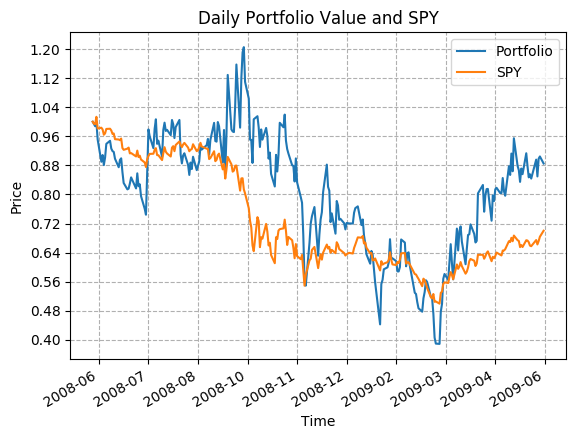
\includegraphics[scale=1]{compare.png}
\end{center}
\end{document}


